\documentclass{article}
\usepackage{enumerate}
\usepackage{amsmath}
\usepackage{amssymb}
\usepackage{graphicx}
\usepackage{subfigure}
\usepackage{geometry}
\usepackage{caption}
\usepackage{stmaryrd}
\geometry{left=3.0cm,right=3.0cm,top=3.0cm,bottom=4.0cm}
\renewcommand{\thesection}{Problem \arabic{section}.}
\title{VP260 PROBLEM SET 6}
\author{Liu Yihao 515370910207}
\date{}
\begin{document}
\maketitle

\section{}
From the class, we know
$$\omega=\frac{qB_0}{m}$$
$$x(t)=0,v_x(t)=0$$
$$y(t)=C_1\sin\omega t-C_2\cos\omega t+\frac{E_0}{B_0}t+C_3$$
$$v_y(t)=C_1\omega\cos\omega t+C_2\omega\sin\omega t+\frac{E_0}{B_0}$$
$$z(t)=C_1\cos\omega t+C_2\sin\omega t+C_4$$
$$v_z(t)=-C_1\omega\sin\omega t+C_2\omega\cos\omega t$$
We can get
$$v_y(0)=C_1\omega+\frac{E_0}{B_0}$$
$$v_z(0)=C_2\omega$$
And apply the initial condition, we obtain
$$-C_2+C_3=0\ \rm{and}\ C_1+C_4=0$$
\begin{enumerate}[(a)]
\item
$$v_y(0)=\frac{E_0}{B_0},C_1=0,C_4=0$$
$$v_z(0)=0,C_2=0,C_3=0$$
$$y(t)=\frac{E_0}{B_0}t,z(t)=0$$
The trajectory is
$$x=z=0,y>0$$
\begin{figure}[h!]
    \centering
    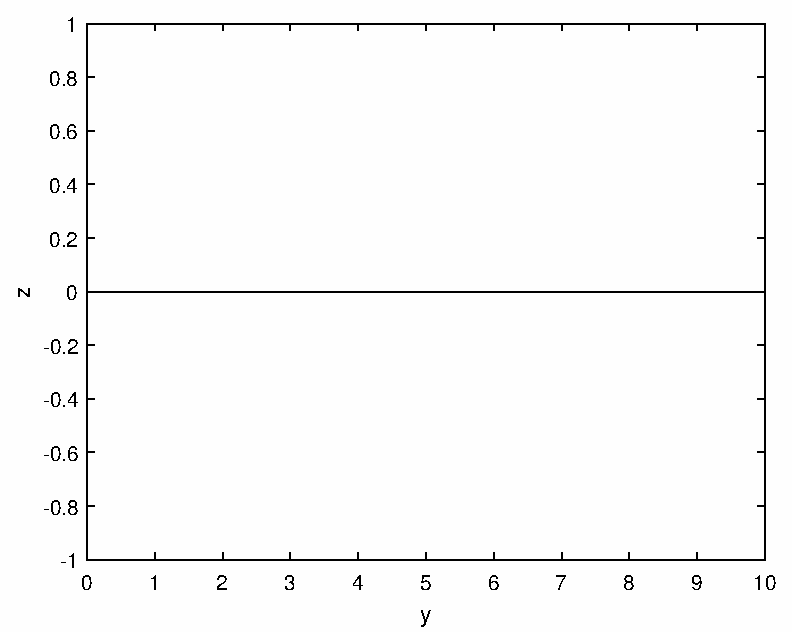
\includegraphics[width=7cm]{1_1.eps}
    \label{fig-1-1}
\end{figure}
\newpage
\item
$$v_y(0)=\frac{E_0}{2B_0},C_1=-\frac{E_0}{2B_0\omega},C_4=\frac{E_0}{2B_0\omega}$$
$$v_z(0)=0,C_2=0,C_3=0$$
$$y(t)=-\frac{E_0}{2B_0\omega}\sin\omega t+\frac{E_0}{B_0}t$$
$$z(t)=-\frac{E_0}{2B_0\omega}(\cos\omega t-1)$$
The trajectory is
$$x=0,\left(y-\frac{E_0}{B_0}t\right)^2+\left(z-\frac{E_0}{2B_0\omega}\right)^2=\left(\frac{E_0}{2B_0\omega}\right)^2$$
\begin{figure}[h!]
    \centering
    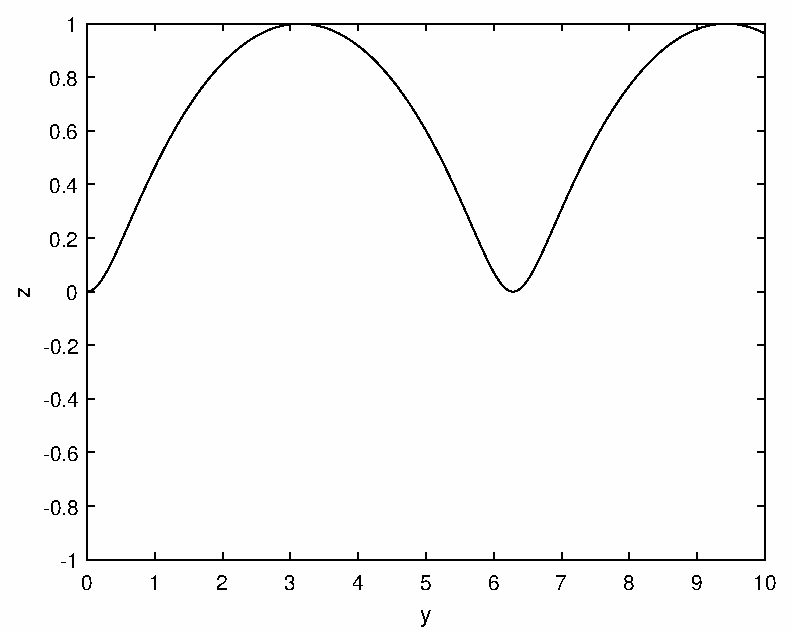
\includegraphics[width=7cm]{1_2.eps}
    \label{fig-1-2}
\end{figure}
\item
$$v_y(0)=\frac{E_0}{B_0},C_1=0,C_4=0$$
$$v_z(0)=\frac{E_0}{B_0},C_2=\frac{E_0}{B_0\omega},C_3=\frac{E_0}{B_0\omega}$$
$$y(t)=-\frac{E_0}{B_0\omega}\cos\omega t+\frac{E_0}{B_0}t+\frac{E_0}{B_0\omega}$$
$$z(t)=\frac{E_0}{B_0\omega}\sin\omega t$$
The trajectory is
$$x=0,\left(y-\frac{E_0}{B_0}t-\frac{E_0}{B_0\omega}\right)^2+z^2=\left(\frac{E_0}{B_0\omega}\right)^2$$
\begin{figure}[h!]
    \centering
    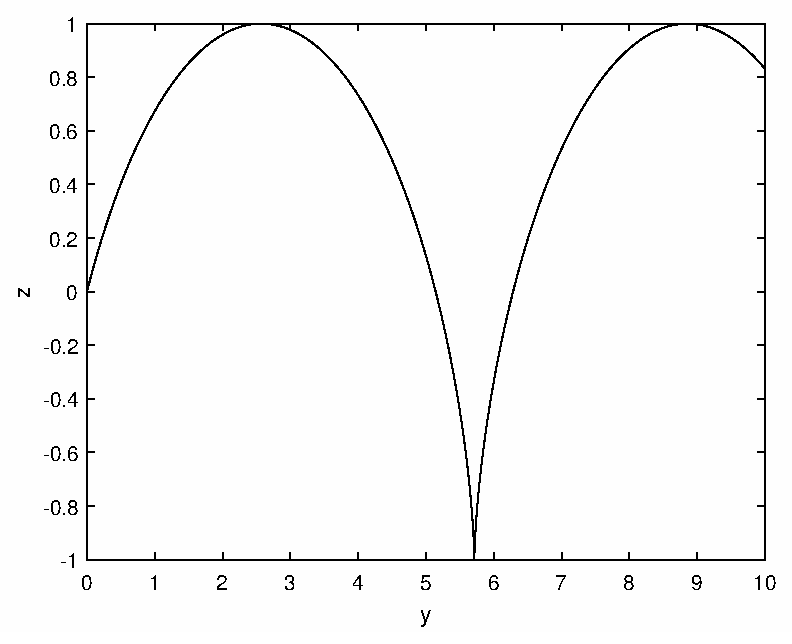
\includegraphics[width=7cm]{1_3.eps}
    \label{fig-1-3}
\end{figure}

\end{enumerate}


\section{}
	$$F=q(E+v\times B)$$
	$$a=\frac{F}{m}=-\frac{qE_0}{m}\hat{n_x}+\frac{qB_0}{m}v_z\hat{n_y}-\frac{qB_0}{m}v_y\hat{n_z}$$
	$$\frac{a_y}{a_z}=\frac{\frac{dv_y}{dt}}{\frac{dv_z}{dt}}=\frac{dv_y}{dv_z}=-\frac{v_z}{v_y}$$
	$$v_ydv_y=-v_zdv_z$$
	Do integral on both side,
	$$\int v_ydv_y=-\int v_zdv_z$$
	$$\frac{1}{2}v_y^2=-\frac{1}{2}v_z^2+C$$
	$$v_y^2+v_z^2=C=v_{0y}^2$$
	$$v_y=v_{0y}\cos\frac{qB_0}{m}t,\ a_y=\frac{qB_0}{m}v_{0y}\sin\frac{qB_0}{m}t$$
	$$v_z=-v_{0y}\sin\frac{qB_0}{m}t,\ a_z=-\frac{qB_0}{m}v_{0y}\cos\frac{qB_0}{m}t$$
	$$v(t)=\left(v_{0x}-\frac{qE_0}{m}t\right)\hat{n_x}+
	\left(v_{0y}\cos\frac{qB_0}{m}t\right)\hat{n_y}-
	\left(v_{0y}\sin\frac{qB_0}{m}t\right)\hat{n_z}$$
	$$r(t)=\left(v_{0x}t-\frac{qE_0}{2m}t^2\right)\hat{n_x}+
	\left(\frac{m}{qB_0}v_{0y}\sin\frac{qB_0}{m}t\right)\hat{n_y}+
	\left(\frac{m}{qB_0}v_{0y}(\cos\frac{qB_0}{m}t-1)\right)\hat{n_z}$$

\section{}
\begin{align*}
F&=\int_{A\to B}I\cdot\overline{dl}\times\overline{B}\\
&=\int_{A\to B}I\cdot\overline{dx}\times\overline{B}+\int_{A\to B}I\cdot\overline{dy}\times\overline{B}\\
&=\int_{A\to B}I\cdot\overline{dx}\times\overline{B}\\
&=IBw
\end{align*}

\section{}
\begin{enumerate}[(a)]
\item
$$J=nqv$$
$$F=NqvB=qvB\cdot nV=BJ\cdot whl$$
$$\Delta p=\frac{F}{S}=JlB$$
\item
$$J=\frac{\Delta p}{lB}=\frac{1.013\times10^5}{3.5\times10^{-2}\cdot2.2}=1.316\times10^5\,\rm{A/m^2}$$
\end{enumerate}

\section{}
\begin{enumerate}[(a)]
\item \ 
\begin{figure}[h!]
    \centering
    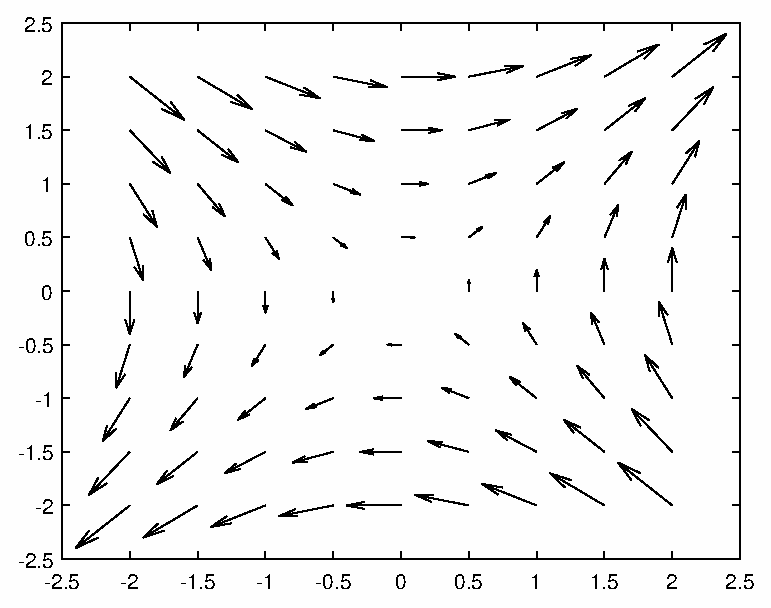
\includegraphics[width=7cm]{5.eps}
    \label{fig-7}
\end{figure}
\item
$$F=\int I\cdot\overline{dl}\times\overline{B}$$
For the left side, $\overline{L}=L\hat{n_y}$, $\overline{B}=\frac{B_0y}{L}\hat{n_x}$
$$F=\int_0^l I\cdot\frac{B_0l}{L}dl(\hat{n_y}\times\hat{n_x})=-\frac{1}{2}IB_0L\hat{n_z}$$
For the right side, $\overline{L}=-L\hat{n_y}$, $\overline{B}=\frac{B_0y}{L}\hat{n_x}+B_0\hat{n_y}$
$$F=\int_0^l I\cdot\frac{B_0l}{L}dl(-\hat{n_y}\times\hat{n_x})=\frac{1}{2}IB_0L\hat{n_z}$$
For the bottom side, $\overline{L}=-L\hat{n_x}$, $\overline{B}=\frac{B_0x}{L}\hat{n_y}$
$$F=\int_0^l I\cdot\frac{B_0l}{L}dl(-\hat{n_x}\times\hat{n_y})=-\frac{1}{2}IB_0L\hat{n_z}$$
For the top side, $\overline{L}=L\hat{n_x}$, $\overline{B}=B_0\hat{n_x}+\frac{B_0x}{L}\hat{n_y}$
$$F=\int_0^l I\cdot\frac{B_0l}{L}dl(\hat{n_x}\times\hat{n_y})=\frac{1}{2}IB_0L\hat{n_z}$$
\item
\begin{align*}
\tau&=\int \overline{r}\times\overline{F}\\
&=\int_0^l I\cdot l\frac{B_0l}{L}dl[\hat{n_y}\times(\hat{n_y}\times\hat{n_x})]
+\int_0^l I\cdot l\frac{B_0l}{L}dl[\hat{n_y}\times(-\hat{n_y}\times\hat{n_x})]
+\int_0^l I\cdot L\frac{B_0l}{L}dl[\hat{n_y}\times(\hat{n_x}\times\hat{n_y})]\\
&=\int_0^l I\cdot L\frac{B_0l}{L}dl\hat{n_x}\\
&=\frac{1}{2}IB_0L^2\hat{n_x}
\end{align*}
\item
\begin{align*}
\tau&=\int \overline{r}\times\overline{F}\\
&=\int_0^l I\cdot l\frac{B_0l}{L}dl[\hat{n_x}\times(\hat{n_x}\times\hat{n_y})]
+\int_0^l I\cdot l\frac{B_0l}{L}dl[\hat{n_x}\times(-\hat{n_x}\times\hat{n_y})]
+\int_0^l I\cdot L\frac{B_0l}{L}dl[\hat{n_x}\times(-\hat{n_y}\times\hat{n_x})]\\
&=\int_0^l I\cdot L\frac{B_0l}{L}dl(-\hat{n_y})\\
&=-\frac{1}{2}IB_0L^2\hat{n_y}
\end{align*}
\item
When it is rotating on one of its edge, the total $\tau$ of two edges perpendicular to the rotating axis is 0, and the $\tau$ on another edge is
$$\tau=L\sin\theta\int_0^l I\cdot \frac{B_0l}{L}dl\hat{n_L}=-\frac{1}{2}IB_0L^2\sin\theta\hat{n_L}$$
Let $|\mu|=IL^2$, $|B|=\frac{1}{2}B_0$ and $\mu\perp B, B\perp L, L\perp\mu$, we obtain
$$\tau=\mu\times B$$

\end{enumerate}


\section{}
\begin{enumerate}[(a)]
\item
\begin{align*}
F&=\int I\cdot\overline{dl}\times\overline{B}\\
&=\int_0^{2\pi} I\cdot Rd\theta\cdot |B|\cos\theta\\
&=I|B|R\int_0^{2\pi}\cos\theta d\theta\\
&=0
\end{align*}
\item
\begin{align*}
\tau&=\int \overline{r}\times\overline{F}\\
&=\int_0^{2\pi} I\cdot Rd\theta\cdot |B|\hat{n_x}\cos\theta \cdot R\cos\theta\\
&=I|B|\hat{n_x}R^2\int_0^{2\pi}\cos^2\theta d\theta\\
&=I\overline{B}\pi R^2
\end{align*}

\end{enumerate}

\section{}
$$B_r(r)\cdot2\pi rh+[B_z(z+h)-B_z(z)]\cdot\pi r^2=0$$
$$B_r(r)=\frac{-\beta h\pi r^2}{2\pi rh}=-\frac{\beta r}{2}$$
\begin{figure}[h!]
    \centering
    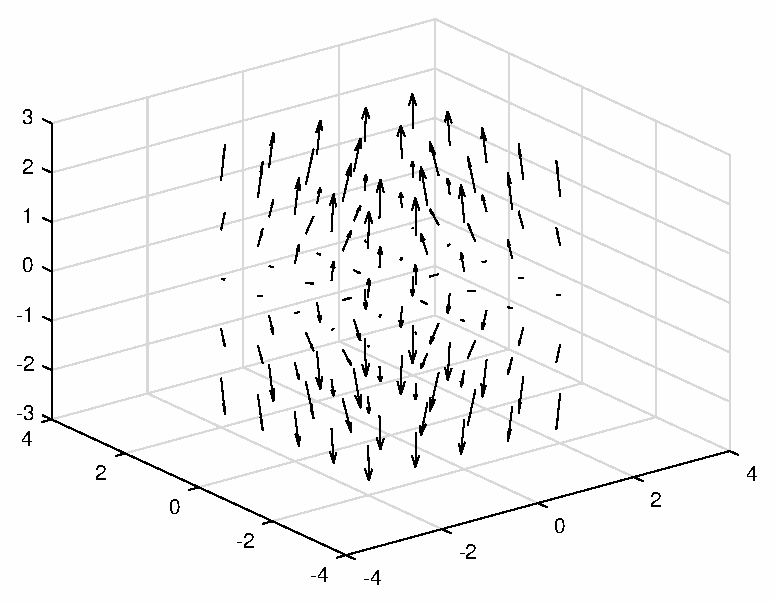
\includegraphics[width=7cm]{7.eps}
    \label{fig-7}
\end{figure}

\end{document}
